\documentclass[aspectratio=169]{beamer}
\usepackage{fao}
\begin{document}

\begin{frame}
  \title{\vspace{-4ex}
    \darkgray SOFIA\raisebox{1pt}{\h{1.5pt}-\h{-1pt}}TAF\\[2ex]
    \normalsize\blue\mdseries\it
    SOFIA analyses organized as TAF repositories on GitHub}
  \author{\vspace{-10ex}\darkgray\bf
    Arni Magnusson, Rishi Sharma, Nicole Tursich}
  \date{\vspace{-1ex}\darkgray FAO\h{1pt}\raisebox{1pt}{-}\h{0.5pt}GFCM Workshop\\[0.3ex]
    Rome, 25 May 2022}
  \titlepage
\end{frame}

% ______________________________________________________________________________

\begin{frame}{\SOFIATAF}
  \begin{itemize}
    \item[]{\darkgray\bf Introduction}
    \comment{Background, Objectives, Open science, Reproducible analyses}\\[3.5ex]
    \item[]{\darkgray\bf Design}
    \comment{Modular, Data flow, Ongoing development}\\[3.5ex]
    \item[]{\darkgray\bf Repositories}
    \comment{Browse, Download, Clone, Hierarchy}\\[3.5ex]
    \item[]{\darkgray\bf TAF}
    \comment{Standard structure, Sequential R scripts, How to run}\\[3.5ex]
    \item[]{\darkgray\bf R packages}
    \comment{SOFIA, TAF, sraplus}\\[3.5ex]
    \item[]{\darkgray\bf SOFIA analyses}
    \comment{Tier 2, Catch, Effort/Index, Priors, Demo}\\[3.5ex]
  \end{itemize}
\end{frame}

% ______________________________________________________________________________

\begin{frame}{Objectives}
  \begin{itemize}
    \item[1. ]{\it Efficiency} \comment{\gray is the ability to edit code in a
      single place to modify a large number of analyses, and to calculate
      top-level summary statistics from a large number of analyses.}\\[3ex]
    \item[2. ]{\it Clarity} \comment{\gray is the ability to easily navigate to
      a specific part of the analysis of a particular stock group and area, and
      to look up a specific result from one or more analyses.}\\[3ex]
    \item[3. ]{\it Traceability} \comment{\gray is the ability to backtrack
      exactly how a specific result was calculated, such as the status of a
      particular stock group in a given area.}\\[3ex]
  \end{itemize}
\end{frame}

\begin{frame}{Objectives (cont)}
  \begin{itemize}
    \item[4. ]{\it Open science} \comment{\gray is the ability to make the R
      scripts available online, along with the input data required for the
      scripts to run, inviting peer review of methodology and scientific
      collaboration.}\\[2.5ex]
    \item[5. ]{\it Reproducibility} \comment{\gray is the ability to run
      analyses on a variety of computers, e.g., a personal Windows laptop or a
      high-performance Linux cluster, to get the exact same result — also when
      the analysis is rerun months or years later.}\\[2.5ex]
    \item[6. ]{\it Quality assurance} \comment{\gray is the design and adoption
      of a workflow that reduces the probability of making human mistakes when
      preparing, modifying, running, and postprocessing the results from
      analyses.}\\[2.5ex]
    \item[7. ]{\it Quality control} \comment{\gray is the ability to identify
      where a human mistake has been made in a given analytical process, so the
      mistake can be located and corrected.}\\[2.5ex]
  \end{itemize}
\end{frame}

% ______________________________________________________________________________

\begin{frame}{\SOFIATAF\ Diagram}
  \centering
  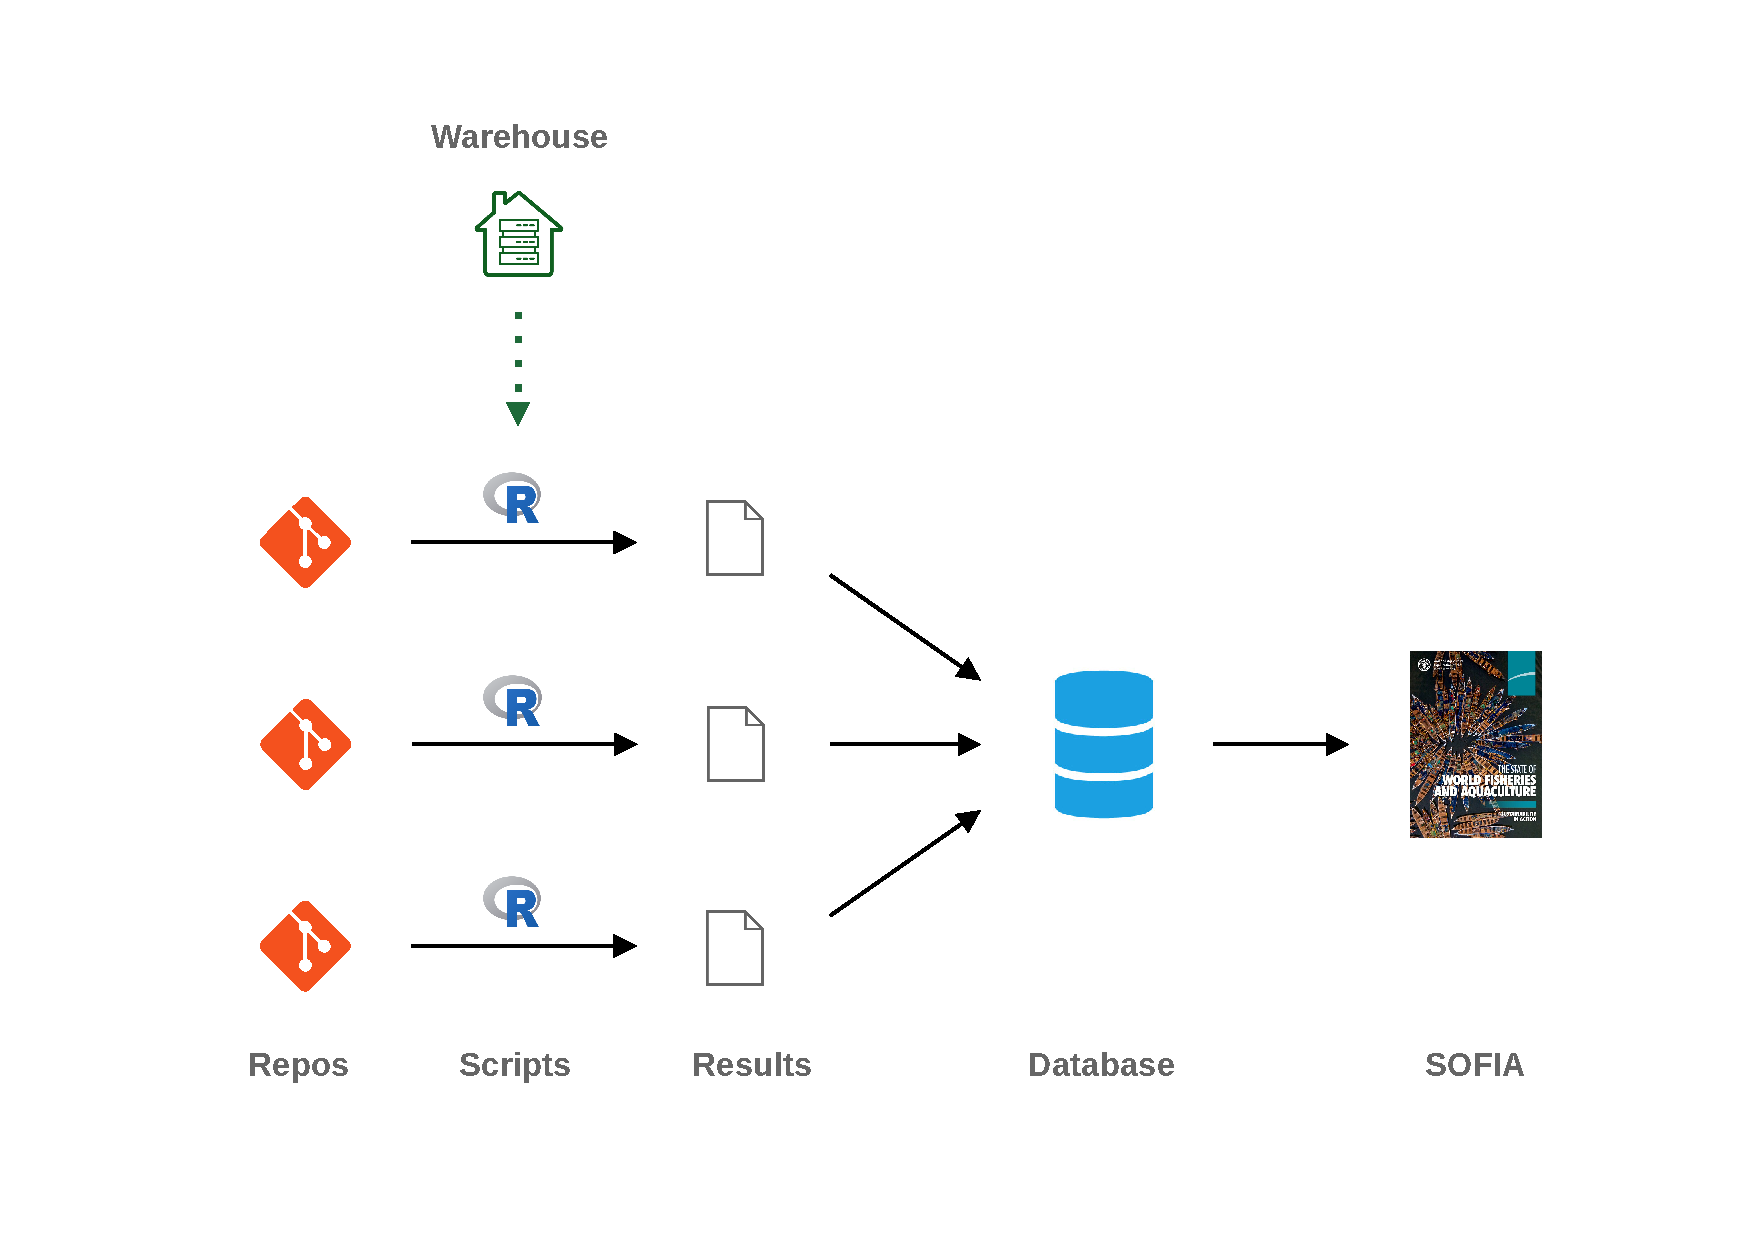
\includegraphics[width=0.6\textwidth]{sofia_taf_diagram}
\end{frame}

\begin{frame}{TAF Diagram}
  \centering
  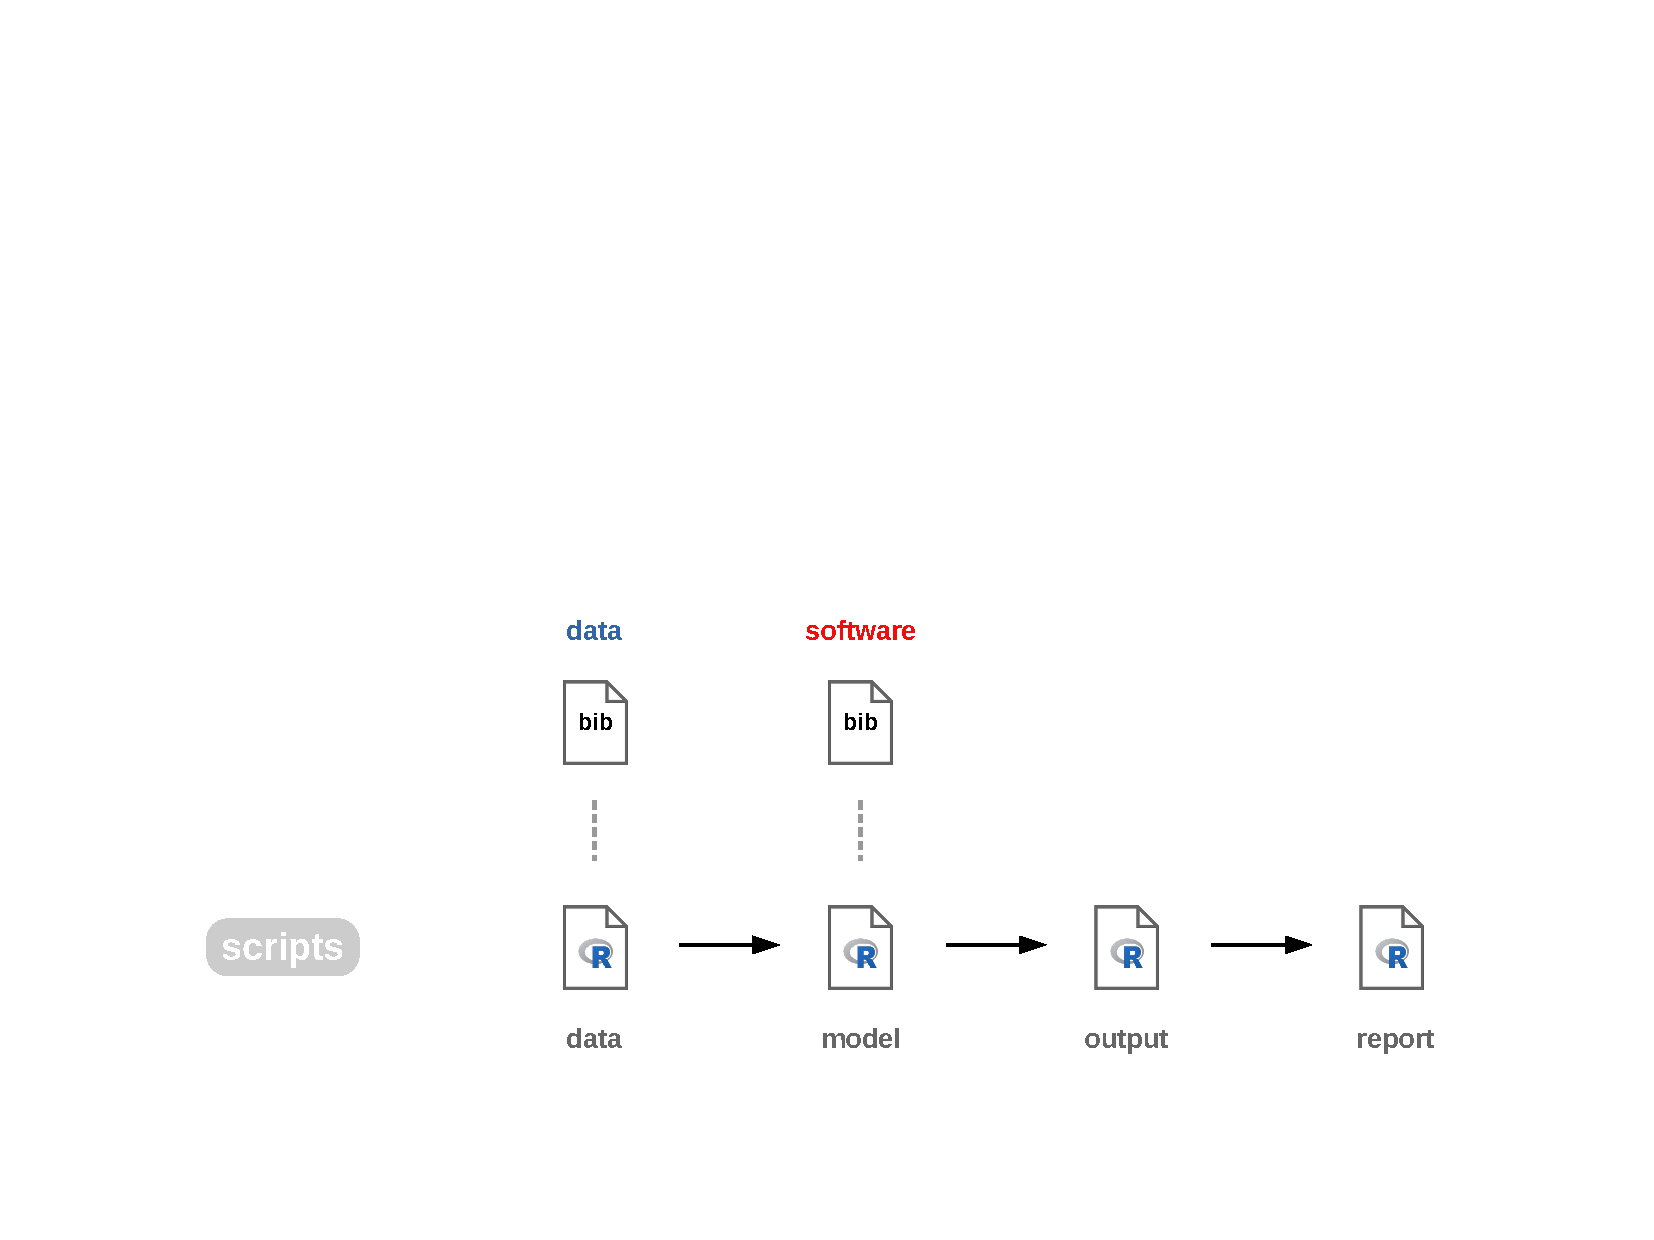
\includegraphics[width=0.8\textwidth]{taf_diagram}
\end{frame}

\begin{frame}{\SOFIATAF\ Directory Structure}
  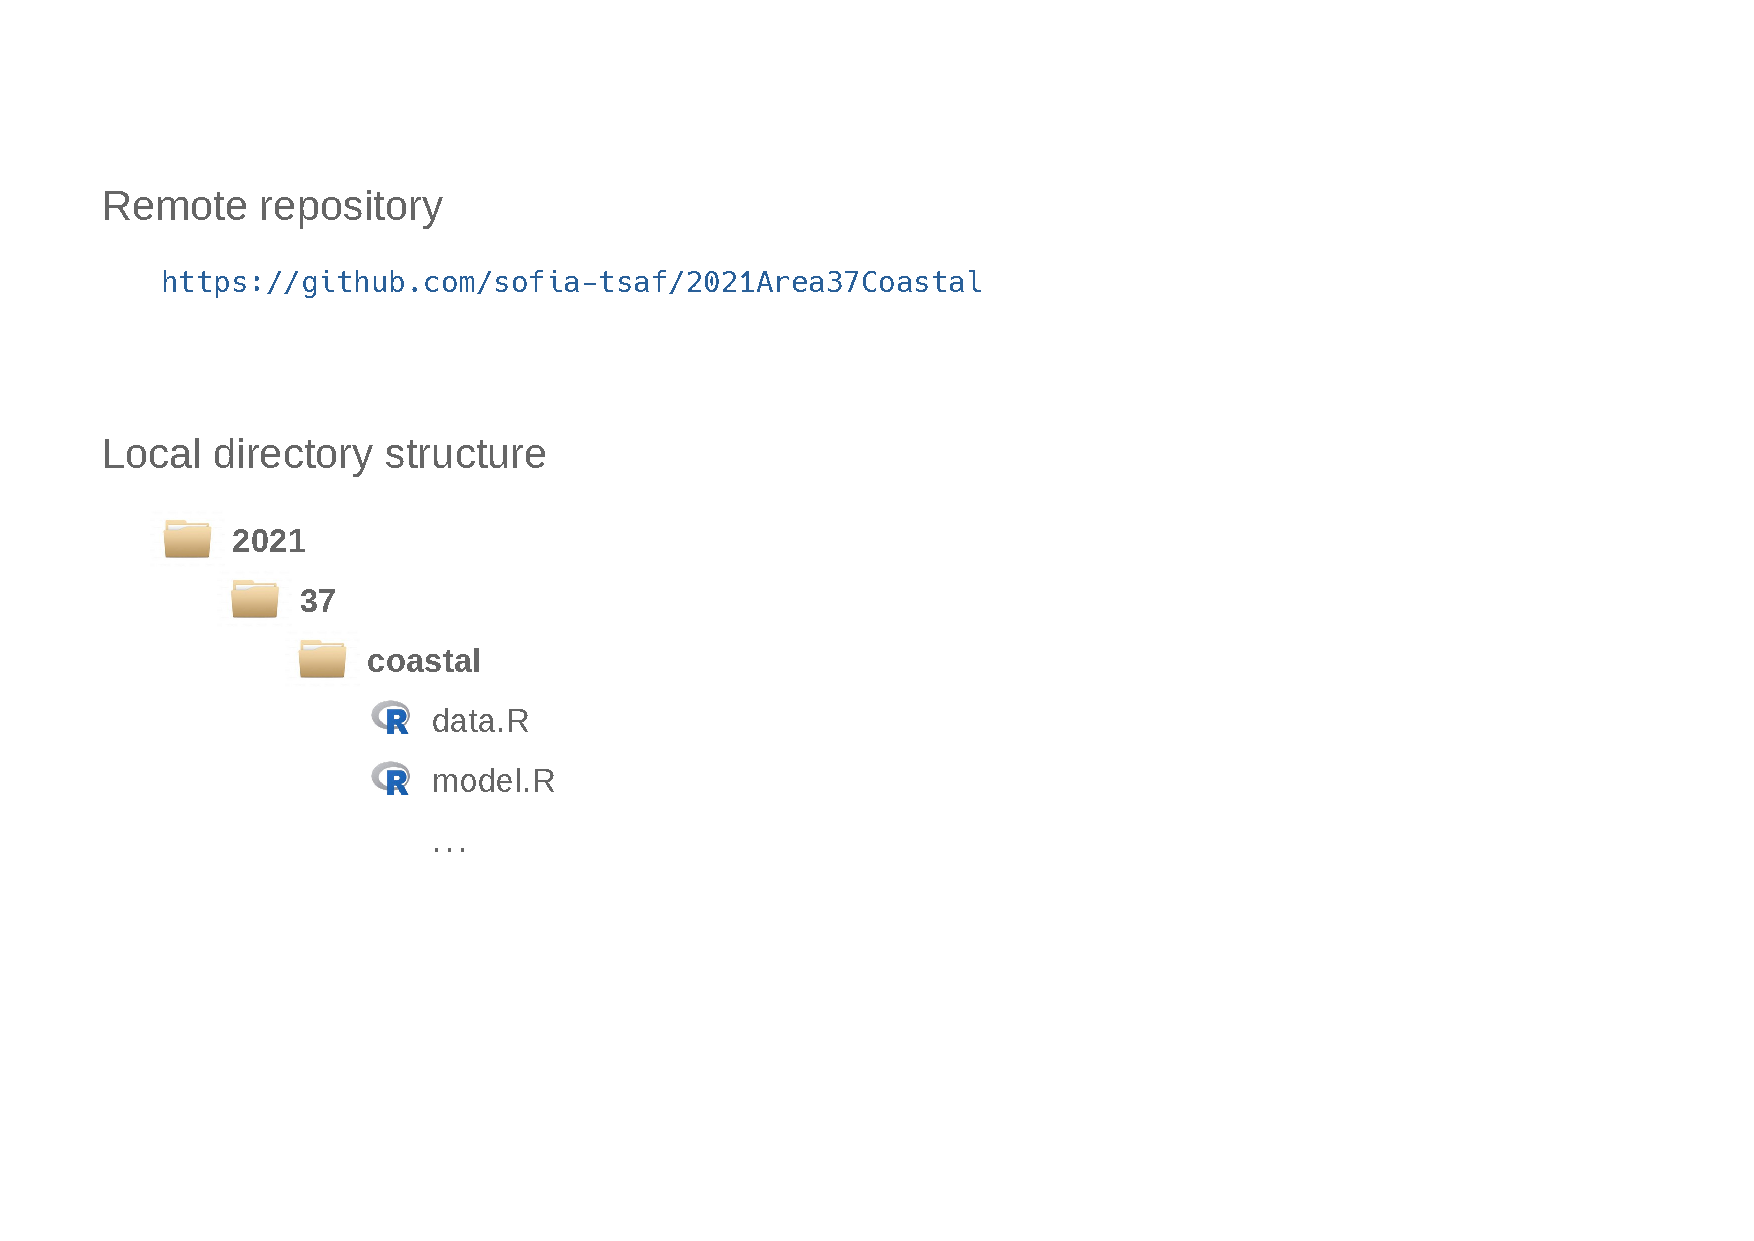
\includegraphics[width=0.55\textwidth]{sofia_taf_dirs}
\end{frame}

% ______________________________________________________________________________

\begin{frame}[fragile]{TAF Scripts}
  \setlength{\tabcolsep}{2ex}
  \begin{tabular}{ll}
    \hline
    Script          & Purpose\I{2.4ex}                                 \\
    \hline
    \verb|data.R|   & Preprocess data, write TAF data tables\I{2.6ex}  \\[0.6ex]
    \verb|model.R|  & Run analysis, write model results                \\[0.6ex]
    \verb|output.R| & Extract
                      results of interest, write TAF output tables     \\[0.6ex]
    \verb|report.R| & Prepare plots and formatted tables               \\[0.4ex]
    \hline
  \end{tabular}
\end{frame}

\end{document}
